\subsection{KNN}
En esta sección definimos:
\begin{itemize}
	\item $k$: cantidad de vecinos a considerar en el algoritmo $kNN$.
\end{itemize}
El análisis sobre el algoritmo $KNN$ ($k$ vecinos más cercanos) se realiza para distintos valores de $k$. La idea detrás de esta elección de la variable busca entender la variación en la efectividad (cantidad de aciertos) del algoritmo.
\\
Para ello variamos $k$ desde $1$ hasta $30$ para ver cual era el comportamiento que se obtenía. Para cada uno de los $k$s realizamos una corrida cross-validarion con $10$ conjuntos.
\\
% El procedimiento de este algoritmo comienza, por cada imágen que queremos averiguar a que dígito pertenece, con su vectorización. Luego resta el resultado a cada uno de los vectores imágen y calcula la norma 2 para saber en cuanto difieren con cada una de las imágenes.
% Todos esos resultados se acumulan en una cola de prioridad que los ordena de menor a mayor, según las diferencias entre la imágen la cual se quiere averiguar a que clase pertenece y todas las imágenes de la base de datos etiquetada.
% \\
% Como siguiente paso se toman los $k$ primeros elementos de la cola de prioridad y se verifica a que dígito se corresponden para luego saber cual es el dígito que recibió mas "votos" y ver si se produjo un acierto o no.
% \subsubsection{Cantidad de vecinos}
% Como ya digimos, para analizar cual es el mejor número de vecinos para el cual el algoritmo $KNN$  da una mayor cantidad de aciertos, optamos por variar la cantidad de $k$ vecinos a tomar.
%Se prueba entonces el algoritmo $KNN$ para los siguientes valores de $k$: $1,2,3,4,...,30$.
%\\
Cada uno de los conjuntos contaba con 4200 imagenes a testear, en los siguientes graficos presentamos algunos de los sets obtenidos:
\\
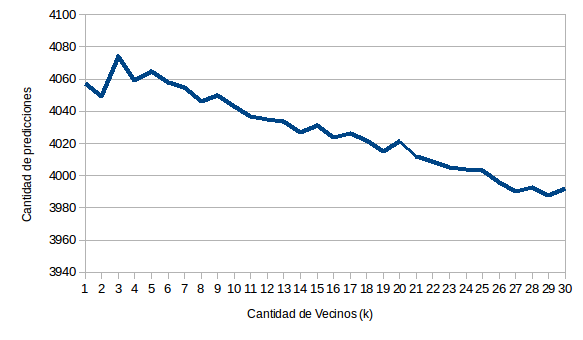
\includegraphics[scale=0.55]{nuevosResultados/knn/1.png}\\

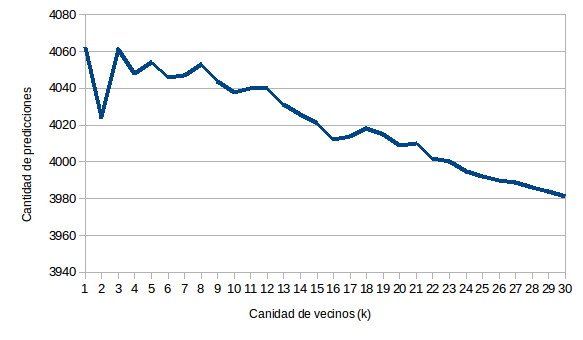
\includegraphics[scale=0.55]{nuevosResultados/knn/2.png}\\

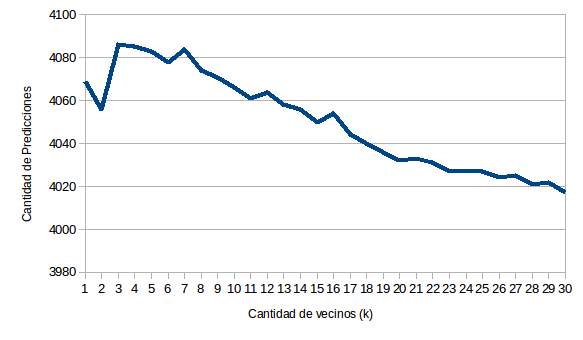
\includegraphics[scale=0.55]{nuevosResultados/knn/3.png}\\

Los resultados son bastante sorprendentes aunque puede verse un patron bastante claro. Para valores muy pequeños de k (k=1,K=2) podemos observar que los resultados son peores que para $k=3$ lo cual no esperabamos que sucediera. Luego para valores mas grandes si se observa lo que nos decía la intuición, tal que para un gran numero de vecinos se empiezan a perder aquellos que son realmente relevantes y las predicciones empiezan a ser peores.
\\
Ademas para estos tests realizamos una medición de tiempos para ver como se comportaba el algoritmo frente a un cambio en la cantidad de vecinos. Los valores promediados para cada $k$ pueden verse en el siguente grafico:

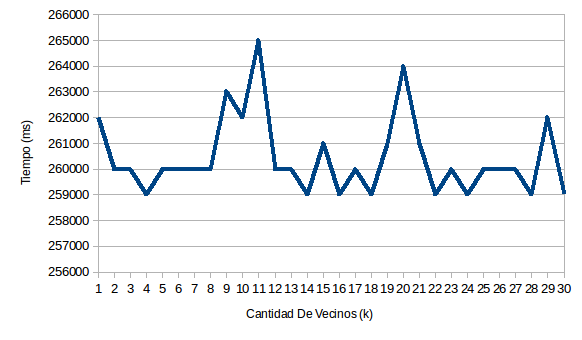
\includegraphics[scale=0.55]{nuevosResultados/knn/1temp.png}\\

Como puede observarse, los tiempos de los algoritmos no se ven muy afectados por la variación en la cantidad de vecinos. Es muy probable que esto se deba a que el algoritmo debe comparar a la imagen que se desea comparar contra un numero muy extenso de imagenes, estan en el mismo orden de magnitud, bla bla...
\completar

Usamos $k=3$ porque es el mejor.

\subsection{PCA}
\subsubsection{Busqueda del mejor valor de $\alpha$}
En esta sección definimos:
\begin{itemize}
	\item $\alpha$: a la cantidad de componentes principales a tomar para el $PCA$.
	\item $k$: cantidad de vecinos a considerar en el algoritmo $kNN$.
\end{itemize}
En primera instancia vamos a utlilizar cross-validation para intentar determinar el mejor $\alpha$ posible. Supondremos en este momento que el mejor $k$ para este caso es el encontrado en la sección anterior (aunque esto podría no ser asi) y luego testearemos si esto es asi o si para el $\alpha$ encontrado existe algun otro $k$ que mejora la cantidad de predicciones del sistema.
\\
Por lo tanto enfocamos nuestro análisis en obtener un valor óptimo de $\alpha$. Para este fin, realizamos partimos el conjunto de datos de entrenamiento en 10 subconjuntos y aplicamos cross-validation. Dado que este parámetro representa la cantidad de componentes principales a tener en cuenta y teniendo en mente el funcionamiento del algoritmo de PCA, es esperable que valores pequeños no sean beneficiosos (teniendo en cuenta que el máximo a considerar es bastante elevado), pero dado que PCA las ordena en base a su relevancia, se alcance un valor óptimo sin necesidad de considerarlas todas. Para esta partición de los datos de entrenamiento con 4200 imagenes para testear, tomamos $\alpha$ desde $1$ hasta $50$ y graficamos lo obtenido:

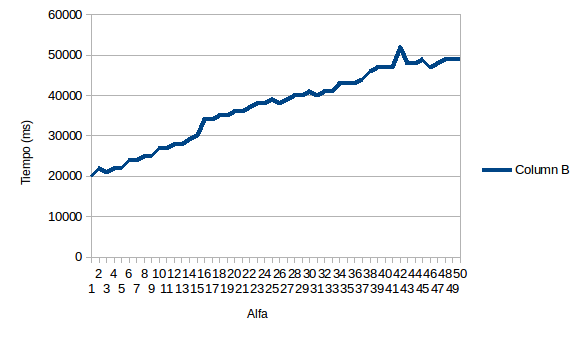
\includegraphics[scale=0.75]{nuevosResultados/pca/pca1.png}\\
Puede verse que para valores pequeños, aumentar en uno el $\alpha$ produce un gran aumento de aciertos. Por ejemplo, considerando el primer set para $\alpha$ igual a $1$ se obtienen $1112$ aciertos, mientras que para $\alpha$ igual a $2$ se obtienen $1680$ aciertos, esto es un $52\%$ mas de aciertos.
\\
Para valores mas grandes de $\alpha$ (al rededor de $\alpha = 12$) esta tendencia empieza estabilizarse. Por ejemplo para $\alpha = 12$ se obtienen $3845$ imagenes correctamente predecidas, pero para $\alpha = 13$ se obtienen $3869$ imagenes correctas, esto es el crecimiento de aciertos es de menos de un $1\%$.
\\
Ademas, para este k-fold medimos los tiempos de ejecución y los promediamos para poder ver de que manera varía la ejecución de los algoritmos en función de $\alpha$:

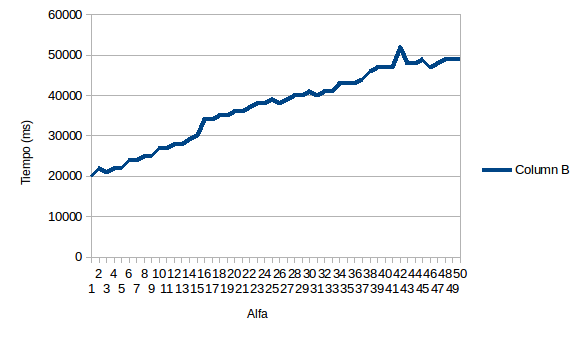
\includegraphics[scale=0.75]{nuevosResultados/pca/pca1.png}\\

En este grafico se puede ver que aumentar el $\alpha$ produce un aumento lineal de los tiempos de ejecución, de lo que se desprende que aumentar la cantidad valores principales no resulta gratuito y tiene cierto costo asociado.
\\
Ademas aumentar de manera desmedida el $\alpha$ puede probocar lo que en machine learning se denomina 'Overfiting'.
\inventarReferencia
\\
Debido a todas las razones expuestas consideramos que con $\alpha$ igual a $14$ será el mejor valor que podemos tomar.
\\

%falta retestear esto de abajo
\subsubsection{Busqueda del mejor valor de $k$}

La segunda prueba a realizar es, fijando un valor de $\alpha$, analizar para que cantidad de vecinos se obtiene la mayor cantidad de aciertos.
\\
Para esto tomamos $\alpha = 14$ volvemos a dividir el conjunto de datos en $10$ sets y realizamos cross validation sobre estos, variando el $k$ desde 1 hasta $30$.
\\
Los resultados obtenidos son los siguientes:
\includegraphics[scale=0.75]{nuevosResultados/pca/pcak1.png}\\

Ademas medimos los tiempos y los promediamos para obtener una idea de como afectan las variaciónes de $k$ a este metodo:

\includegraphics[scale=0.75]{nuevosResultados/pca/pcak1temp.png}\\


